% 第四章 生成场景的质量验证
\chapter{生成场景的质量验证}
\section{实验设置}
\textbf{(1)测试数据集构成} \par
测试数据集旨在综合自动驾驶场景的多样性和复杂性,涵盖多种典型场景类别,如直行障碍、转弯障碍、变道、超车、闯红灯、无保护左转、右转、以及交叉路口协商等。这些场景类别覆盖了自动驾驶车辆在实际道路环境中可能遇到的关键交互情况,具备较高的代表性和实用价值。
数据集中的场景描述以自然语言形式呈现,且包括一定比例的模糊性描述,以模拟真实世界中驾驶员或其他交通参与者行为的不可预测性。场景描述的模糊性设计有助于测试生成系统在面对不精确指令时的处理能力,确保系统能够适应并生成符合要求的复杂交通场景。\\
\indent\textbf{(2)对比基线选择依据} \par
在评估生成场景的质量时,本研究选用了两种具有代表性的方法作为基线进行对比:
基于规则的方法(Rule-based):该方法通过定义明确的逻辑和规则来生成场景,具有较好的可解释性,适合处理结构化和预定义的任务。然而,在面对复杂和模糊的自然语言描述时,其灵活性和适应性较差。
基于GPT-4.0的方法:借助于大型语言模型的生成能力,能够生成丰富多样的场景。尽管其在场景生成的多样性方面具有优势,但可能在生成的场景物理合规性和逻辑一致性上存在一定不足,尤其是在处理复杂交通情境时。
选择这两种基线的目的是为了从不同角度评估本研究方法在生成场景质量、效率以及对复杂和模糊指令的鲁棒性方面的优势。\\
\indent\textbf{(3)硬件平台与评估指标} \par
硬件平台:本实验使用联想Y900P高性能笔记本电脑。该平台配置了多核的 Intel Core i9 处理器,能够高效处理复杂的计算任务,确保场景生成的实时性和响应速度。此外,配备的专业级显卡为图形处理和并行计算任务提供了强大支持,尤其是在大规模场景生成过程中。系统还配备大容量内存和高速固态硬盘(SSD),确保数据处理和存储高效、稳定。
评估指标:为了全面评估生成场景的质量,本研究采用以下几个关键指标:
场景生成时间:该指标衡量生成一个场景所需的时间,反映了系统的效率。较短的生成时间有助于提高测试的灵活性和响应速度。
场景物理合规性:评估生成场景是否符合物理约束条件,如车辆的最大加速度、最小转弯半径等。物理合规性确保了场景的真实性,生成的场景能真实反映自动驾驶系统的实际驾驶条件。
场景逻辑一致性:检查场景中各元素之间的逻辑关系是否合理,确保生成的场景符合法律规定的交通规则。逻辑一致性是验证场景真实性和可接受性的核心标准。
场景多样性:统计生成场景的类型和数量,衡量系统的多样性和生成能力。多样性高的系统能为自动驾驶系统提供更广泛的测试场景,从而有效覆盖更多潜在的驾驶情况。
碰撞率:在仿真环境中运行生成的场景,并统计发生碰撞的频率。碰撞率反映了生成场景的安全性,较低的碰撞率意味着生成的场景能够较好地模拟真实世界中的安全驾驶环境。




\section{生成效果展示(示例)}

\subsection{场景一:摩托车和汽车在红绿灯前等待信号}
\indent 一辆摩托车和一辆汽车在红绿灯前等待信号。\\

\begin{figure}[H]
	\centering
	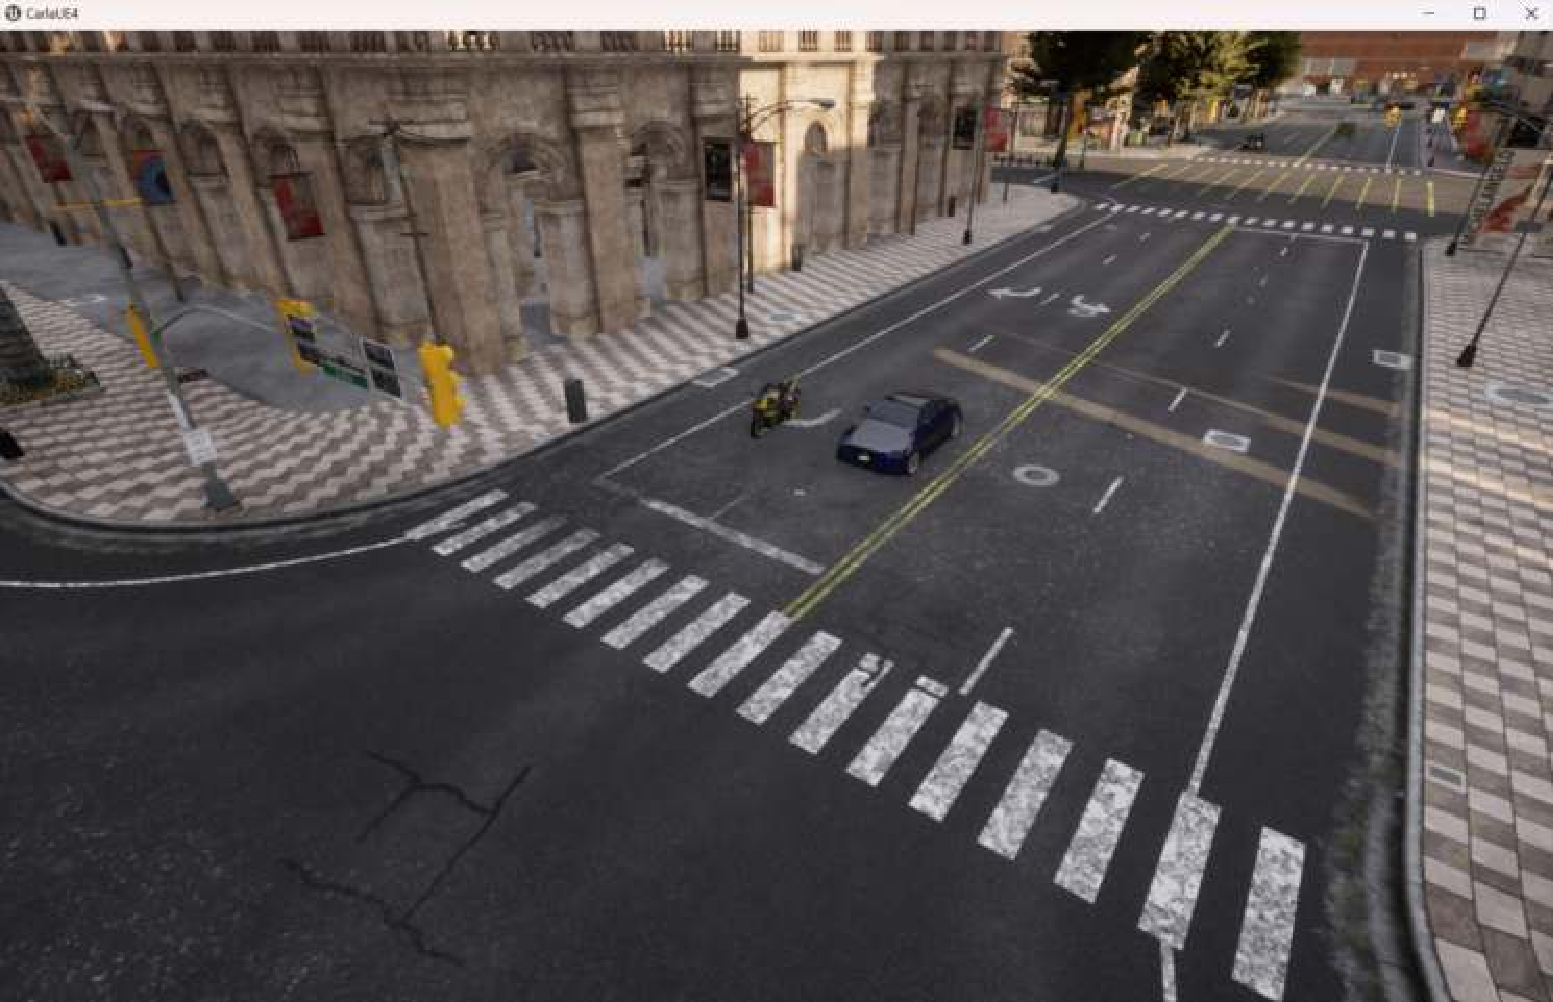
\includegraphics[width=1.0\textwidth]{"images/1.png"}
	\caption{摩托车与汽车在红绿灯前等待信号的场景截图}
	\label{fig:redlight_motorbike_car}
\end{figure}

\subsection{场景二:自我车辆在夜晚穿越道路}
\indent 在夜晚,一些自我车辆正在穿越道路,街道上的路灯微弱地照亮着周围环境,远处偶尔可以看到其他车辆的车灯闪烁。\\

\begin{figure}[H]
	\centering
	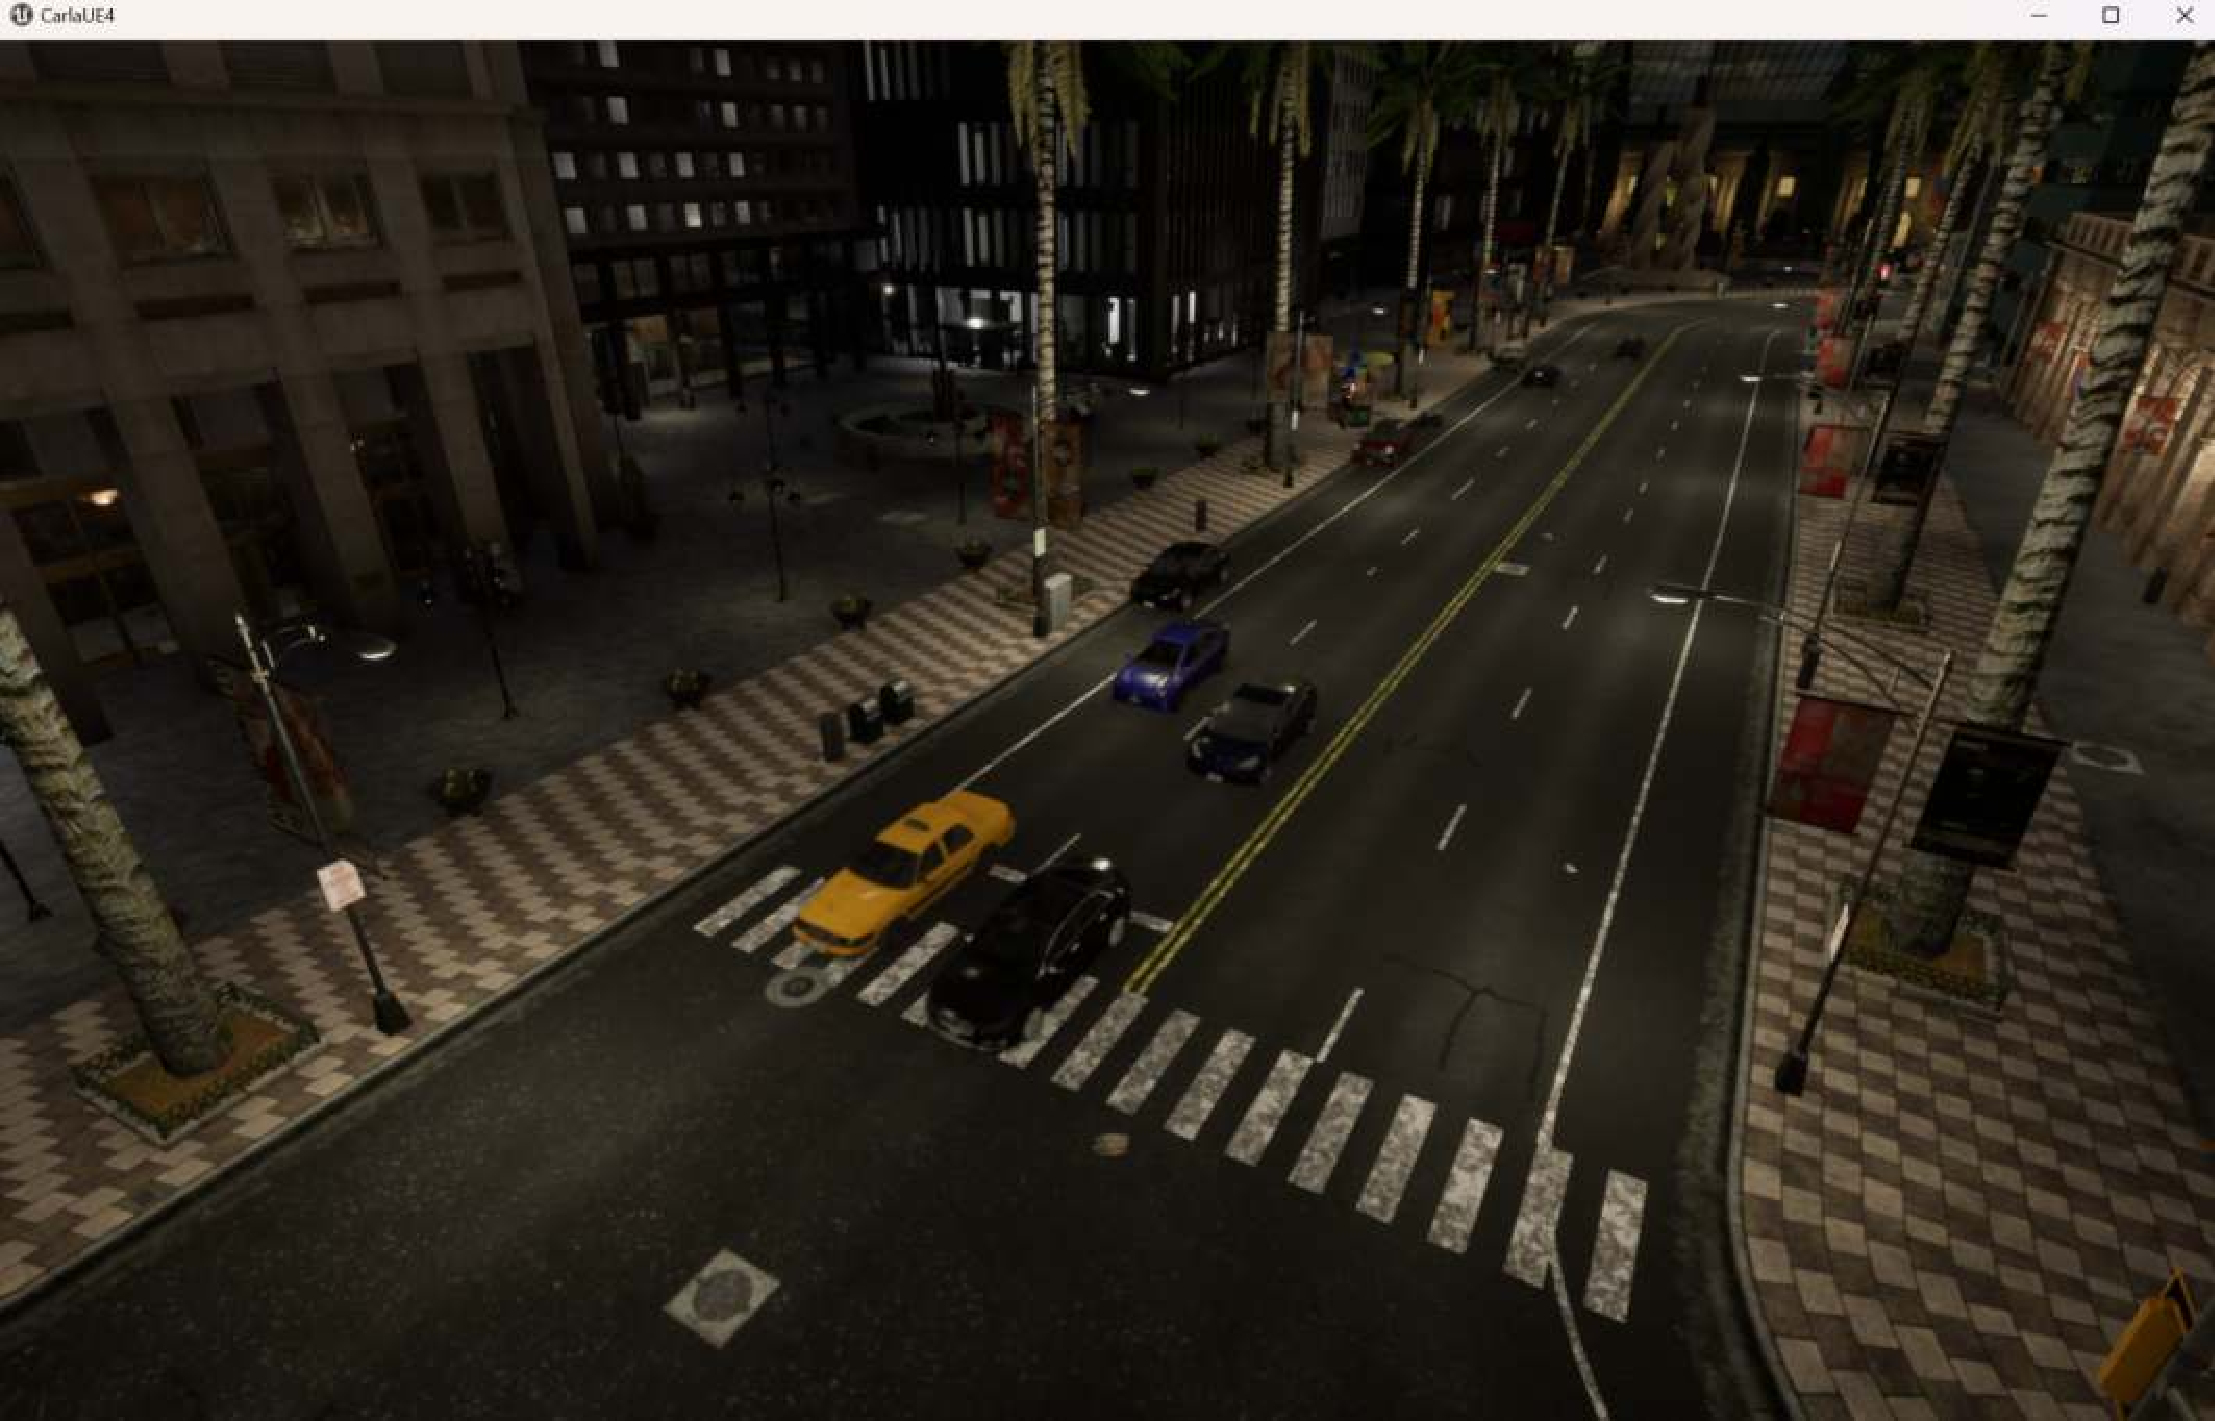
\includegraphics[width=1.0\textwidth]{"images/2.png"}
	\caption{自我车辆在夜晚穿越道路的场景截图}
	\label{fig:night_self_driving_cross}
\end{figure}

\subsection{场景三:自我车辆在夜晚红绿灯前等待信号}
\indent 在夜晚,一些自我车辆在红绿灯前等待信号,而在另一方向,自我车辆正在通行,车灯的光芒穿过昏暗的街道。\\

\begin{figure}[H]
	\centering
	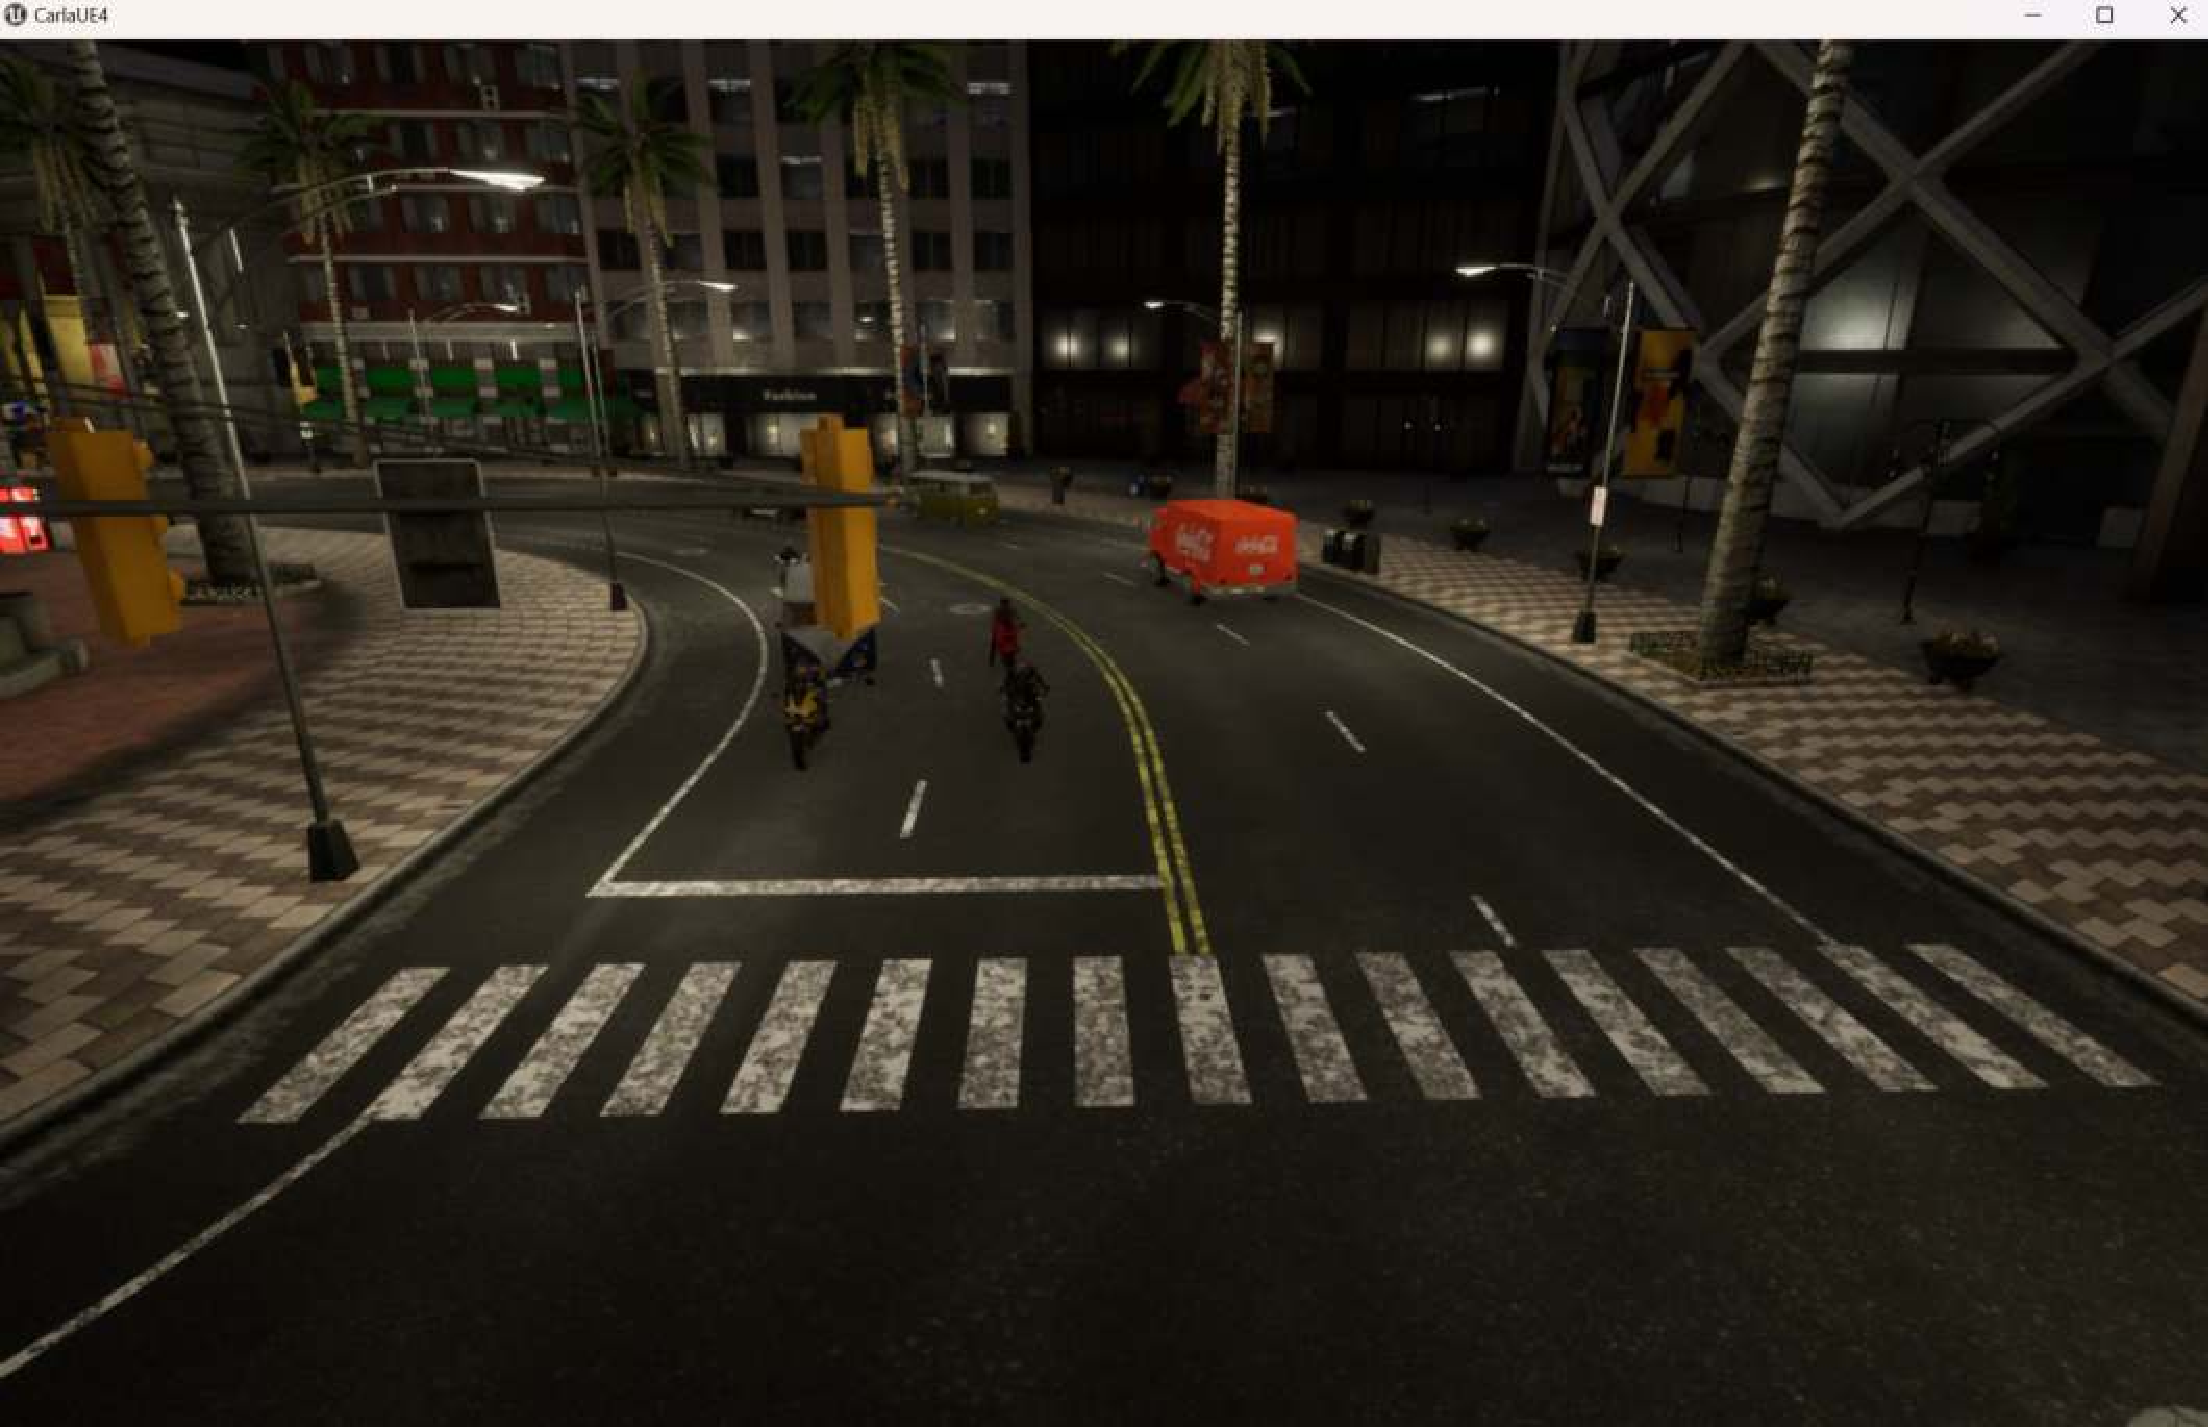
\includegraphics[width=1.0\textwidth]{"images/4.png"}
	\caption{自我车辆在夜晚红绿灯前等待信号的场景截图}
	\label{fig:night_redlight_cross}
\end{figure}

\subsection{场景四:行人横穿直行道路}
\indent 自我车辆在笔直的道路上行驶时,一名行人突然从右前方横穿过来,并在自我车辆接近时突然停下。\\

\begin{figure}[H]
	\centering
	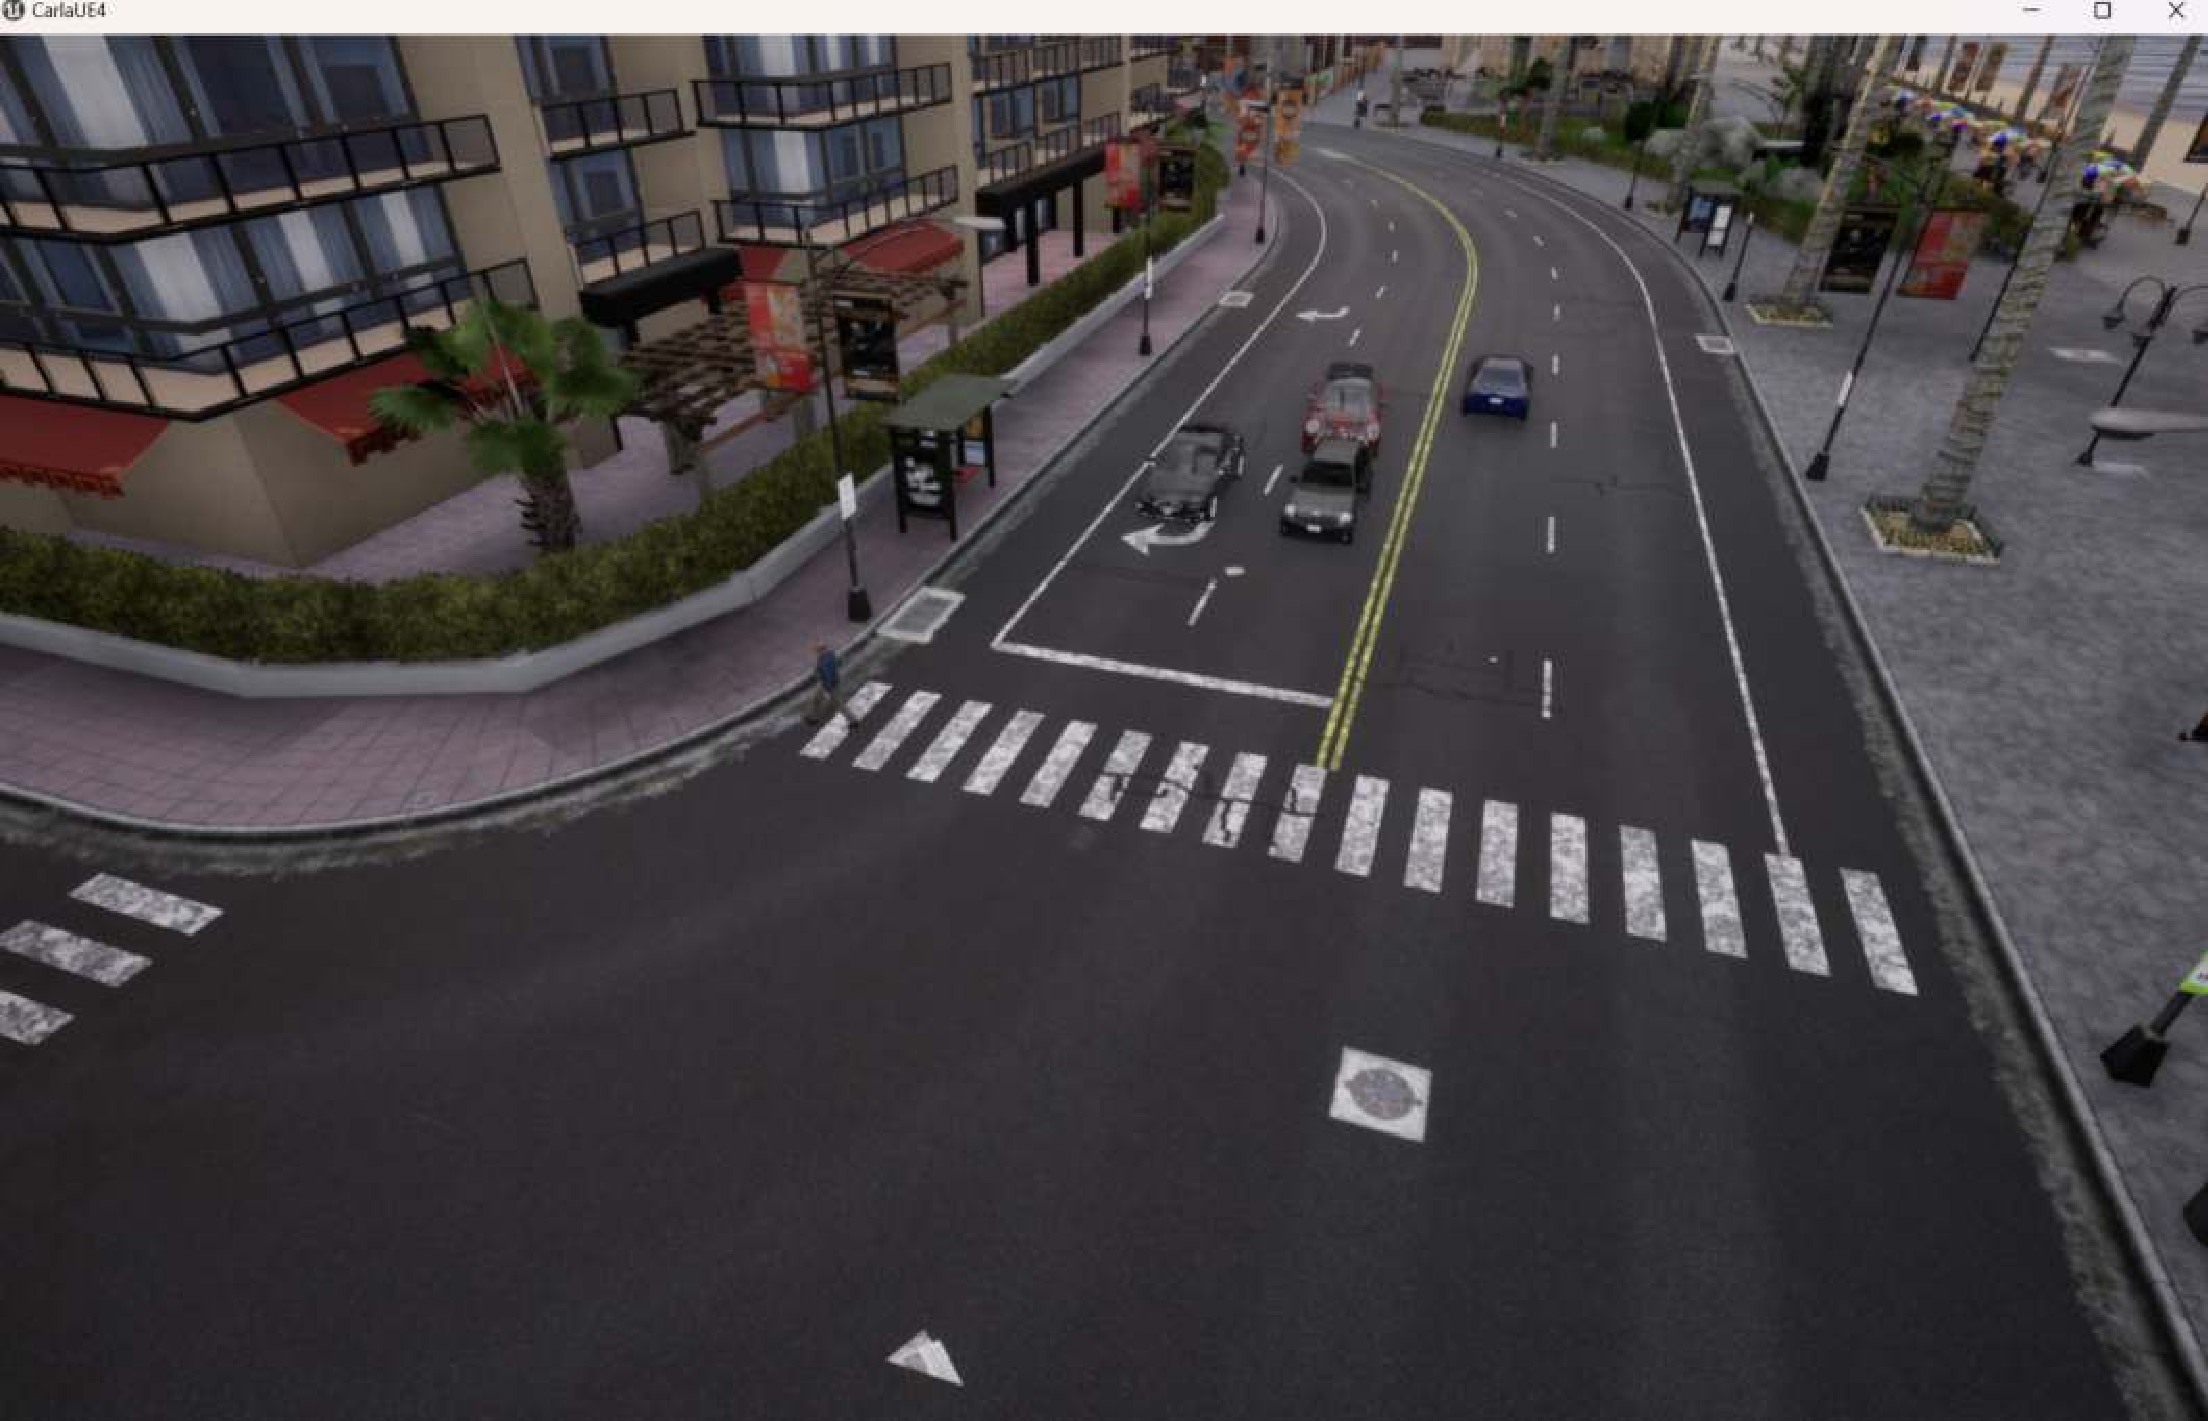
\includegraphics[width=1.0\textwidth]{"images/5.png"}
	\caption{行人横穿直行道路的场景截图}
	\label{fig:pedestrian_crossing}
\end{figure}

\section{实验总结}

本章着重描述了基于自然语言生成三维交通场景的核心流程:“语言描述 → 场景代码生成 → 仿真构建”。此流程展示了如何通过自然语言输入、自动脚本生成与仿真执行的技术路径,实现复杂三维交通场景的高效构建。

\begin{itemize}
	\item \textbf{语言描述的输入与解析}:整个流程的第一步是通过 \texttt{scenario\_descriptions.txt} 文件获取自然语言描述。每条描述代表了一个特定的交通场景,包括交通参与者的类型、数量、初始位置、行为意图等信息。用户通过直观的语言输入定义了所需的场景特征。系统通过 \texttt{retrieve.py} 脚本对输入的自然语言进行语义解析。解析的目标是从文本中识别出场景的关键元素,比如车辆的种类、行驶方向、速度,甚至是动态行为(如超车、停车、避让等)。该步骤主要依赖自然语言处理(NLP)技术,通过文本特征提取与词汇映射,将模糊的语言信息转换为有结构的场景要素。
	
	\item \textbf{场景代码的自动生成}:一旦自然语言描述被解析,系统通过预设的规则与模板生成符合 Scenic 语法规范的场景脚本。Scenic 是一种针对三维仿真场景描述的语言,其特点是灵活且适用于动态场景建模。系统根据输入的描述生成的代码包含了场景中参与者的初始化设置(如车辆的位置、速度、运动轨迹等)以及可能的动态行为(如交通参与者的交互、变道、超车等)。生成的 Scenic 脚本是可执行的,并能传递给 Scenic 编译器作为输入文件。此阶段的自动化程度高,能够在大部分场景下自动生成相应的场景代码,减少了人工干预的需要。
	
	\item \textbf{仿真场景的构建与执行}:生成的 Scenic 场景脚本会被传递到仿真平台,主要是 CARLA,通过 Scenic-CARLA 接口执行。CARLA 是一个开源的自动驾驶仿真平台,它能够根据场景脚本中的设置构建出真实感强、动态可控的三维仿真场景。在此过程中,系统会依照 Scenic 脚本中的配置加载地图、部署交通参与者(如汽车、行人等)、设置场景初始状态(如天气、时间、环境条件等)。此外,仿真平台还根据脚本中的动态行为设定实时执行参与者的运动轨迹与交互。例如,当脚本指定一辆车在道路上缓慢行驶并让行时,CARLA 仿真平台会根据脚本设置准确模拟该行为,确保生成的仿真场景在空间和行为上都符合预期。
	
	\item \textbf{系统流程特性与优势}:整个“语言描述 → 场景代码生成 → 仿真构建”的流程展现了系统的自动化处理能力,尤其是自然语言到仿真场景代码生成的桥接。通过 \texttt{retrieve.py} 脚本,用户能够快速通过文本输入生成三维交通场景,减少了手动构建仿真场景的工作量。此外,该流程支持生成复杂场景和动态交互行为,能够精准还原交通系统中的各种交互情境,如追尾、避让、变道等,为自动驾驶系统的测试与评估提供了有效的支持。
	
\end{itemize}
\begin{figure}[H]
	\centering
	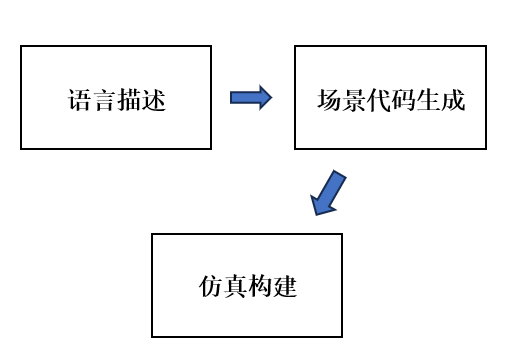
\includegraphics[width=1.0\textwidth]{"images/流程图1.pdf"}
	\caption{从自然语言描述到仿真场景构建的流程图}
	\label{fig:flowchart}
\end{figure}